\documentclass[a4paper]{article}
\usepackage[margin=2cm]{geometry}
\setlength\parindent{0pt}
\setlength{\parskip}{1em}

\usepackage{amsmath}
\usepackage{amssymb}
\usepackage{amsthm}
\usepackage{amsfonts}
\usepackage{bm}
\usepackage{commath}

% Column vectors
\newcount\colveccount
\newcommand*\colvec[1]{
	\global\colveccount#1
	\begin{pmatrix}
		\colvecnext
	}
	\def\colvecnext#1{
		#1
		\global\advance\colveccount-1
		\ifnum\colveccount>0
			\\
			\expandafter\colvecnext
		\else
		\end{pmatrix}
	\fi
}

% Vector norm
\newcommand{\Norm}[1]{
	\left\lVert#1\right\rVert
}

% Inner product
\newcommand{\innerp}[2]{
	\langle #1,#2 \rangle
}

\usepackage{tikz}
\usepackage{tikz-3dplot}
\usetikzlibrary{arrows, calc}
\tikzset{vector/.style={->, >=stealth, very thick, cap=round}}
\definecolor{col0}{HTML}{FFFFFF}
\definecolor{col1}{HTML}{FF7878}
\definecolor{col2}{HTML}{51B5F8}
\definecolor{col3}{HTML}{68E1AA}
\definecolor{col4}{HTML}{B869EA}
\definecolor{col5}{HTML}{FF5500}
\definecolor{col6}{HTML}{FF7878}
\definecolor{col7}{HTML}{FF7500}
\definecolor{col8}{HTML}{FF4F93}

\usepackage{float}

\title{Calculations}

\begin{document}
\maketitle

%% ----- Particle-Particle ----- %%
\section{Collision of Two Spherical Particles Moving at Constant Velocities}
\subsection{Time to Collision}
Two spherical particles with radii $R_{1}$ and $R_{2}$, have initial positions $\bm{x}^{0}_{1}$ and $\bm{x}^{0}_{2}$ and move with constant velocities $\bm{v}_{1}$ and $\bm{v}_{2}$, respectively. At what time, if at all, will they collide?

\begin{figure}[H]
	\centering
	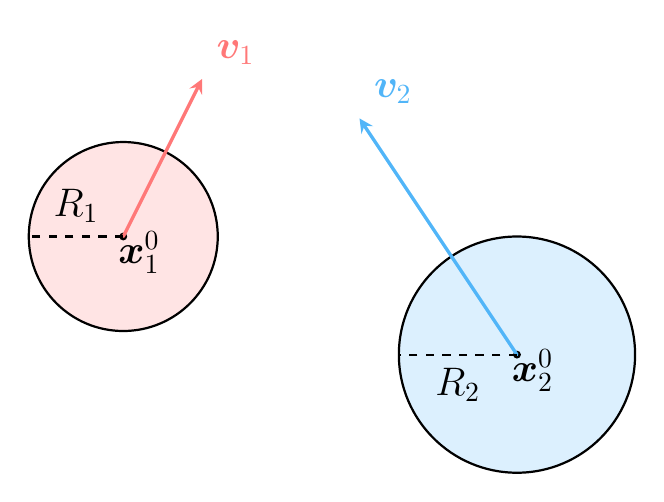
\begin{tikzpicture}
		\Large
		\coordinate (x1) at (0,0);
		\draw[thick, fill=col1!20] (x1) circle (1.2);
		\fill[black] (x1) circle (0.05);
		\draw[vector, col1] (x1) -- ++(1,2) node [above right] {$\bm{v}_{1}$};
		\draw[dashed, thick] (x1) -- ++(-1.2,0) node [midway, above] {$R_{1}$};
		\node at (0.2,-0.2) {$\bm{x}^{0}_{1}$};
		
		\coordinate (x2) at (5,-1.5);
		\draw[thick, fill=col2!20] (x2) circle (1.5);
		\fill[black] (x2) circle (0.05);
		\draw[vector, col2] (x2) -- ++(-2,3) node [above right] {$\bm{v}_{2}$};
		\draw[dashed, thick] (x2) -- ++(-1.5,0) node [midway, below] {$R_{2}$};
		\node at ($(x2)+(0.2,-0.2)$) {$\bm{x}^{0}_{2}$};
	\end{tikzpicture}
\end{figure}

The position of particle 1 as a function of time is
\begin{equation}
	\bm{x}_{1}(t) = \bm{x}^{0}_{1} + \bm{v}_{1}t,
	\label{eq:p1_pos}
\end{equation}
The position of particle 2 as a function of time is identical, i.e.
\begin{equation}
	\bm{x}_{2}(t) = \bm{x}^{0}_{2} + \bm{v}_{2}t.
	\label{eq:p2_pos}
\end{equation}
Therefore, the distance $\bm{r}(t)$ between the particles is
\begin{equation}
	\bm{r}(t) = \bm{x}_{1}(t) - \bm{x}_{2}(t) = \bm{x}^{0}_{1} + \bm{v}_{1}t - \bm{x}^{0}_{2} - \bm{v}_{2}t,
	\label{eq:distance_vec}
\end{equation}
or in explicit vector form
	\begin{align}
	\bm{r}(t) &= \colvec{3}{x^{0}_{1}+v^{x}_{1}t - x^{0}_{2}+v^{x}_{2}t}{y^{0}_{1}+v^{y}_{1}t - y^{0}_{2}+v^{y}_{2}t}{z^{0}_{1}+v^{z}_{1}t - z^{0}_{2}+v^{z}_{2}t}\nonumber\\
	&= \colvec{3}{\left(x^{0}_{1}-x^{0}_{2}\right)-\left(v^{x}_{1}-v^{x}_{2}\right)t}{\left(y^{0}_{1}-y^{0}_{2}\right)-\left(v^{y}_{1}-v^{y}_{2}\right)t}{\left(z^{0}_{1}-z^{0}_{2}\right)-\left(v^{z}_{1}-v^{z}_{2}\right)t}\nonumber\\
	&= \colvec{3}{\Delta x_{0}-\Delta v^{x}t}{\Delta y_{0}-\Delta v^{y}t}{\Delta z_{0}-\Delta v^{z}t}.
		\label{eq:distance_explicit}
	\end{align}

	The square of the norm of $\bm{r}(t)$ is thus
	\begin{align}
		\Norm{r}^{2} &= \left( \Delta x_{0}-\Delta v^{x}t \right)^{2} + \left( \Delta x_{0}-\Delta v^{x}t \right)^{2} + \left( \Delta x_{0}-\Delta v^{x}t \right)^{2}\nonumber\\
		&= \left(\Delta x_{0}\right)^{2} - 2\Delta x_{0}\Delta v^{x}t + \left(\Delta v^{x}\right)^{2}t^{2} + \cdots\nonumber\\
		&= \left(\Delta x_{0}\right)^{2} + \left( \Delta y_{0} \right)^{2} + \left( \Delta z_{0} \right)^{2} - 2\left( \Delta x_{0}\Delta v^{x} + \Delta y_{0}\Delta v^{y} + \Delta z_{0}\Delta v^{z} \right)t + \left(\left( \Delta v^{x} \right)^{2} + \left( \Delta v^{y} \right)^{2} + \left( \Delta v^{z} \right)^{2}\right)t^{2}\nonumber\\
		&= \Norm{\Delta \bm{x}_{0}}^{2} - 2\innerp{\Delta\bm{x}_{0}}{\Delta\bm{v}}t + \Norm{\Delta \bm{v}}^{2}t^{2}.
		\label{eq:norm_square_dist}
	\end{align}

	The times $t_{1,2}$ for which the particles collide can be calculated by solving equation \ref{eq:norm_square_dist} for the case
	\begin{equation}
		\Norm{r}^{2} = \left(R_{1}+R_{2}\right)^{2} = R^{2},
		\label{eq:collision}
	\end{equation}
	i.e. when the distance between the particles is the sum of their radii.

	Using the quadratic formula,
	\begin{align}
		t_{1,2} &= \frac{2\innerp{\Delta\bm{x}_{0}}{\Delta\bm{v}}\pm\sqrt{4\innerp{\Delta\bm{x}_{0}}{\Delta\bm{v}}^{2} - 4\Norm{\Delta\bm{v}}^{2}\left( \Norm{\Delta\bm{x}_{0}}^{2}-R^{2} \right)}}{2\Norm{\Delta\bm{v}}^{2}}\nonumber\\
		&= \frac{\innerp{\Delta\bm{x}_{0}}{\Delta\bm{v}}\pm\sqrt{\innerp{\Delta\bm{x}_{0}}{\Delta\bm{v}}^{2} - \Norm{\Delta\bm{v}}^{2}\left( \Norm{\Delta\bm{x}_{0}}^{2}-R^{2} \right)}}{\Norm{\Delta\bm{v}}^{2}}.
		\label{eq:quad_formula}
	\end{align}

	The condition for which a collision will happen is therefore
	\begin{equation}
		\innerp{\Delta\bm{x}_{0}}{\Delta\bm{v}}^{2} \geq \Norm{\Delta\bm{v}}^{2}\left( \Norm{\Delta\bm{x}_{0}}^{2}-R^{2} \right).
		\label{eq:if_collision}
	\end{equation}

\subsection{Veclocity Change}

%% ----- Particle-Wall ----- %%
\section{Collision of a Spherical Particle and a Planar Wall}
\subsection{Definition of a Planar Wall}
A plane can be defined by a point and a direction normal to the plane. However, we wish to use only a finite part of the plane. We therefore define a wall using a point $\bm{\sigma}$ and two orthogonal vectors $\bm{d}_{1}$ and $\bm{d}_{2}$:

\begin{figure}[H]
	\centering
	\tdplotsetmaincoords{110}{20}
	\begin{tikzpicture}[tdplot_main_coords]
		\Large
		\draw[thick, fill=col3!30] (-3,-3,0) -- (3,-3,0) -- (3,3,0) -- (-3,3,0) -- cycle;
		\draw (0,-0.5,0) -- (0.5,-0.5,0) -- (0.5,0,0);
		\draw[vector, col4] (0,0,0) -- node [midway, below] {$\bm{d}_{1}$} (3,0,0);
		\draw[vector, col5] (0,0,0) -- node [midway, left] {$\bm{d}_{2}$} (0,-3,0);
		\filldraw (0,0,0) circle (0.1) node [below left] {$\bm{\sigma}$};
	\end{tikzpicture}
\end{figure}

The normal to the wall surface can then be defined as
\begin{equation}
	\bm{\hat{n}} = \frac{\bm{d}_{1} \times \bm{d}_{2}}{\Norm{\bm{d}_{1} \times \bm{d}_{2}}}.
	\label{eq:surfce_norm}
\end{equation}

\subsection{Time to Collision}
The distance $d$ between a spherical particle and a wall can be calculated as the distance between its center (a point) and the plane of which the wall is a part of. This distance is the projection of the vector $\bm{x}-\bm{\sigma}$ onto $\bm{\hat{n}}$:

\begin{figure}[H]
	\centering
	\tdplotsetmaincoords{110}{20}
	\begin{tikzpicture}[tdplot_main_coords]
		\Large
		\draw[thick, dashed, cap=round, fill=col3, opacity=0.3] (-3,-3,0) -- (3,-3,0) -- (3,3,0) -- (-3,3,0) -- cycle;
		\coordinate (x) at (2,-2,2);
		\coordinate (x_) at ($(x)-(0,0,2)$);
		\draw[vector, thick, col2] (0,0,0) -- (x);
		\draw[thick, densely dotted, col1!60] (x) -- (x_) node [midway, right] {$d$};
		\node[draw=none, shape=circle, fill=col1, inner sep=1.5pt] at (x) {};
		\node[right of=x, xshift=-5mm, text=col1] {$\bm{x}$};
		\draw[thick, col1!60] (x_) -- (0,0,0);
		\filldraw (0,0,0) circle (0.1) node [below left] {$\bm{\sigma}$};
		\draw[vector] (0,0,0) -- (0,0,1) node [left, yshift=-2mm] {$\bm{\hat{n}}$};
	\end{tikzpicture}
\end{figure}

Using the dot product, it can be written as
\begin{equation}
	d = \innerp{\bm{x}-\bm{\sigma}}{\bm{\hat{n}}},
	\label{eq:d_value}
\end{equation}
since $\Norm{\bm{\hat{n}}} = 1$.

In order to have a concise notation for the following part, we define two new concepts:
\begin{enumerate}
	\item \textbf{Squared vector}:
	\begin{equation}
		\bm{v}=\colvec{4}{v_{1}}{v_{2}}{\vdots}{v_{n}} \Rightarrow \bm{v}^{2} \equiv \colvec{4}{v_{1}^{2}}{v_{2}^{2}}{\vdots}{v_{n}^{2}}.
		\label{eq:sqr_vec}
	\end{equation}

	\item \textbf{Speical triple product}: the triple product of three vectors $\bm{u},\ \bm{v},\ \bm{w}$ is
	\begin{equation}
		\left[ \bm{u},\bm{v},\bm{w} \right] \equiv \sum\limits_{i=1}^{n} u_{i}v_{i}w_{i}.
		\label{eq:triple_prod}
	\end{equation}
\end{enumerate}

\subsection{Velocity Change}
\begin{figure}[H]
	\centering
	\tdplotsetmaincoords{110}{20}
	\begin{tikzpicture}[tdplot_main_coords]
		\Large
		\draw[thick, dashed, cap=round, fill=col3, opacity=0.3] (-3,-3,0) -- (3,-3,0) -- (3,3,0) -- (-3,3,0) -- cycle;
		\draw[vector, col2] (0,0,0) -- (2,1,3) node [midway, above left] {$\bm{v}'$};
		\draw[vector, col4] (0,0,0) -- (0,0,1) node [midway, above right] {$\hat{\bm{n}}$};
		\draw[vector, col1] (-2,-1,3) -- (0,0,0) node [midway, above right] {$\bm{v}$};
	\end{tikzpicture}
\end{figure}
The projection of $\bm{v}$ onto $\bm{\hat{n}}$ is
\begin{equation}
	\text{proj}_{\bm{\hat{n}}}\bm{v} = \innerp{\bm{v}}{\bm{\hat{n}}}\bm{\hat{n}},
	\label{eq:proj_v_n}
\end{equation}
and on a direction orthogonal to $\bm{\hat{n}}$ is
\begin{equation}
	\bm{v} - \innerp{\bm{v}}{\bm{\hat{n}}}\bm{\hat{n}}.
	\label{eq:proj_v_perp_n}
\end{equation}
$\bm{v}$ can be reconstructed from these two components,
\begin{equation}
	\bm{v} = \innerp{\bm{v}}{\bm{\hat{n}}}\bm{\hat{n}} + \bm{v} - \innerp{\bm{v}}{\bm{\hat{n}}}\bm{\hat{n}}.
	\label{eq:v_by_components}
\end{equation}
Similarly, $\bm{v}'$ has the $\bm{\hat{n}}$ opposite and equal in magnitude to that of $\bm{v}$, and the orthogonal component equal to that of $\bm{v}$, yielding
\begin{align}
	\bm{v}' &= -\innerp{\bm{v}}{\bm{\hat{n}}}\bm{\hat{n}} + \bm{v} - \innerp{\bm{v}}{\bm{\hat{n}}}\bm{\hat{n}}\nonumber\\
	&= \bm{v} - 2\innerp{\bm{v}}{\bm{\hat{n}}}\bm{\hat{n}}.
	\label{eq:v_prime}
\end{align}
\end{document}
